\documentclass{exam}
\usepackage[utf8]{inputenc}
\usepackage{lmodern}
\usepackage{microtype}

% \usepackage[parfill]{parskip}
\usepackage[dvipsnames]{xcolor}
\usepackage{amsmath}
\usepackage{amsfonts}
\usepackage{amsthm}
\usepackage{siunitx}
\DeclareSIUnit\year{yr}
\DeclareSIUnit\foot{ft}
\DeclareSIUnit\litre{\liter}

\usepackage{skull}

\usepackage{pgfplots}
\usepgfplotslibrary{polar}
\pgfplotsset{compat=1.11}
\usepackage{graphicx}
\usepackage{sidecap}
\sidecaptionvpos{figure}{c}
\usepackage{float}
\usepackage{gensymb}
\usepackage{tkz-euclide}
\usetkzobj{all}
\usepackage{commath}
\usepackage{hyperref}
\usepackage{enumitem}
\usepackage{wasysym}
\usepackage{multicol}
\usepackage{mathtools}
\usepackage{tcolorbox}
\usepackage{tabularx}
\usepackage[version=4]{mhchem}
\usepackage{changepage}
\usepackage{listings}
\lstset{basicstyle=\ttfamily\linespread{0.8}\small}

\renewcommand*{\thefootnote}{\fnsymbol{footnote}}

\newtheorem*{thm}{Theorem}
\newtheorem*{iden}{Identity}
\newtheorem*{lemma}{Lemma}
\newtheorem{obs}{Observation}
\theoremstyle{definition}
\newtheorem*{defn}{Definition}
\newtheorem*{ex}{Example}
\newtheorem{con}{Construction}
\newtheorem*{alg}{Algorithm}

\newtheoremstyle{break}
  {\topsep}{\topsep}%
  {\itshape}{}%
  {\bfseries}{}%
  {\newline}{}%
\theoremstyle{break}
\newtheorem*{bthm}{Theorem}

% russian integral
\usepackage{scalerel}
\DeclareMathOperator*{\rint}{\scalerel*{\rotatebox{17}{$\!\int\!$}}{\int}}

% \DeclareMathOperator*{\rint}{\int}

\pgfplotsset{vasymptote/.style={
    before end axis/.append code={
        \draw[densely dashed] ({rel axis cs:0,0} -| {axis cs:#1,0})
        -- ({rel axis cs:0,1} -| {axis cs:#1,0});
    }
}}

% \pointsinrightmargin
\boxedpoints
\pointname{}

\newcommand{\questioA}{\question[\texttt{\textbf{\color{Cerulean} A}}]}
\newcommand{\questioM}{\question[\texttt{\textbf{\color{PineGreen} M}}]}
\newcommand{\questioE}{\question[\texttt{\textbf{\color{WildStrawberry} E}}]}
\newcommand{\questioS}{\question[\texttt{\textbf{\color{Goldenrod} S}}]}
\newcommand{\questioO}{\question[\texttt{\textbf{\color{BurntOrange} O}}]}

\newcommand{\parA}{\part[\texttt{\textbf{\color{Cerulean} A}}]}
\newcommand{\parM}{\part[\texttt{\textbf{\color{PineGreen} M}}]}
\newcommand{\parE}{\part[\texttt{\textbf{\color{WildStrawberry} E}}]}
\newcommand{\parS}{\part[\texttt{\textbf{\color{Goldenrod} S}}]}
\newcommand{\parO}{\part[\texttt{\textbf{\color{BurntOrange} O}}]}

\newcommand{\subparA}{\subpart[\texttt{\textbf{\color{Cerulean} A}}]}
\newcommand{\subparM}{\subpart[\texttt{\textbf{\color{PineGreen} M}}]}
\newcommand{\subparE}{\subpart[\texttt{\textbf{\color{WildStrawberry} E}}]}
\newcommand{\subparS}{\subpart[\texttt{\textbf{\color{Goldenrod} S}}]}
\newcommand{\subparO}{\subpart[\texttt{\textbf{\color{BurntOrange} O}}]}

\newcommand{\mainHeader}[2]{\section*{NCEA Level 2 Mathematics\\#1. #2}}
\newcommand{\mainHeaderHw}[2]{\section*{NCEA Level 2 Mathematics (Homework)\\#1. #2}}

\begin{document}

\mainHeaderIntg{19}{Differential Equations}
Many physical problems can be expressed by writing different rates of change in terms of each other. For example,
for a spring pulled a distance $ x $ away from its equilibrium point we have
\begin{displaymath}
  \od[2]{x}{t} = -kx
\end{displaymath}
for some constant $ k $; and for a falling stone at distance $ r $ from the centre of the Earth, we have
\begin{displaymath}
  \od[2]{r}{t} = -\frac{K}{r^2}
\end{displaymath}
where $ K $ is some constant. These kinds of equations are known as \textbf{differential equations}.

Suppose $ \od{y}{x} = f(x) g(y) $. It would be nice if we could find $ y $ in terms of $ x $ only. This
is in fact possible, using substitution:
\begin{align*}
  \dod{y}{x} &= f(x) g(y) \\
  \Rightarrow \frac{1}{g(y)} \dod{y}{x} &= f(x)\\
  \Rightarrow \rint \frac{1}{g(y)} \dod{y}{x} \dif{x} &= \rint f(x) \dif{x}.
\end{align*}

Now, let $ G(y) $ be an antiderivative of $ \frac{1}{g(y)} $ (with respect to $ y $). By the chain rule, then,
\begin{displaymath}
  \od{}{x} G(y) = \frac{1}{g(y)} \od{y}{x}
\end{displaymath}
and so
\begin{displaymath}
  \rint \frac{1}{g(y)} \od{y}{x} \dif{x} = G(y) = \rint \frac{1}{g(y)} \dif{y}.
\end{displaymath}
Hence we have
\begin{displaymath}
  \rint \frac{1}{g(y)} \dif{y} = \rint f(x) \dif{x}
\end{displaymath}
This way of solving differential equations is called \textbf{separation of variables}.

\begin{ex}
  Suppose we know that $ y\od{y}{x} = e^x $. Then we can separate the variables:
  \begin{align*}
    \rint y \dif{y} &= \rint e^x \dif{x}\\
    \Rightarrow \frac{1}{2} y^2 &= e^x + C\\
    \Rightarrow y^2 &= 2e^x + C.
  \end{align*}
  If we know that the curve passes through $ (0,0) $, then $ 0 = 2e^0 + C $ and $ C = -2 $, so $ y^2 = 2e^x - 2 $.

  To check our answer, let us now use implicit differentiation to differentiate this curve. We have $ 2y \od{y}{x} = 2e^x $ so and $ y \od{y}{x} = e^x $
  as expected: our solution is correct.
\end{ex}

If we have a differential equation of the form $ \od{y}{x} + A(x)y + B(x) = 0 $ for any functions $ A $ and $ B $, then for
every point $ (x_0,y_0) $ in the plane, there exists a unique solution $ f $ whose graph $ y = f(x) $ passes through $ (x_0, y_0) $.

  \clearpage
\begin{ex}
  Suppose that $ r(\theta) $ is implicitly defined by $ \od{r}{\theta} = r \sin \theta $ with the condition $ r(\pi) = e $.
  Separating variables, we have $ \rint \frac{\dif{r}}{r} = \rint \sin \theta \dif{\theta} $; so $ \ln \abs{r} = -\cos \theta + C $
  and therefore $ r = Ke^{-\cos \theta} $ for some constant $ K $. But $ e = Ke^{-\cos \pi} = Ke^0 = K $; so $ r(\theta) = e e^{-\cos \theta} = e^{1 - \cos \theta} $.
  Graphing this:
  \begin{center}
    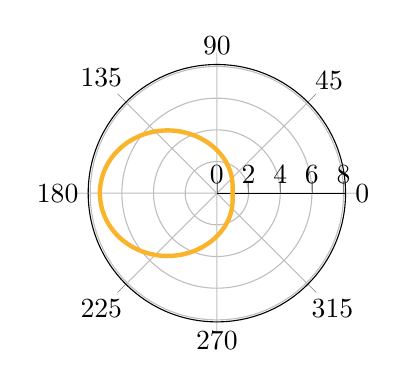
\begin{tikzpicture}
      \begin{polaraxis}[width=0.4\textwidth]
        \addplot[domain=0:360,samples=360,color=Dandelion,style=ultra thick]{e^(1-cos(x))};
      \end{polaraxis}
    \end{tikzpicture}
  \end{center}
\end{ex}

\subsection*{Questions}
\begin{questions}
  \questioM Find $ y $ in terms of $ x $ in each case, if each curve passes through $ (1,1) $:
    \begin{multicols}{2}
    \begin{parts}
      \part $ \od{y}{x} = yx $
      \part $ \od{y}{x} + x = yx $
      \part $ \od{y}{x} + y = yx $
      \part $ \sqrt{y} \od{y}{x} = \frac{1}{x} $
      \part $ \od{y}{x} = (x + 2)^2 $
      \part $ \od{y}{x} = \frac{y^2 + 1}{2y} e^x $
      \part $ \od{y}{x} = x\cos^2 y $
      \part $ \od{y}{x} = \sin x \tan y $
      \part $ 2y \od{y}{x} = x^3 + 2x + 1 $
      \part $ \sin y \od{y}{x} = 3x $
      \part $ \od{y}{x} = \frac{x(e^{x^2} + 2)}{6y^2} $
    \end{parts}
    \end{multicols}
  \questioE
    \begin{parts}
      \part Show that one antiderivative of $ f(x) = x \sin x \dif{x} $ is $ F(x) = \sin x - x \cos x $.
      \part Find $ y(\pi) $ if $ y(0) = \pi $ and
        \begin{displaymath}
          \od{y}{\theta} = \theta y \sin \theta.
        \end{displaymath}
    \end{parts}
  \questioE Newton's law of cooling states that the rate of heat loss of a body is directly proportional to the difference in the
            temperatures between the body and its surroundings; in other words, if the temperature of the body at time $ t $ is $ T $
            and the ambient temperature is $ T_{\infty} $ then $ \od{T}{t} = -k(T - T_{\infty}) $ (where $ k $ is some constant.)
    \begin{parts}
      \part A loaf of bread is taken from the oven at a temperature of \SI{400}{\celsius} and is set down on a bench in an area
            with an ambient temperature of \SI{20}{\celsius}. It is found that it takes ten minutes for the loaf to cool to half
            its initial temperature. How many minutes will it take for the loaf to cool to \SI{30}{\celsius}?
      \part A detective is called to the scene of a crime where a dead body has just been found. She arrives on the scene at
            10:23 pm and begins her investigation. Immediately, the temperature of the body is taken and is found to be \SI{24}{\celsius}.
            The detective checks the programmable thermostat and finds that the room has been kept at a constant \SI{20}{\celsius} for
            the past 3 days.

            After evidence from the crime scene is collected, the temperature of the body is taken once more and found to be \SI{22}{\celsius}.
            This last temperature reading was taken exactly one hour after the first one. Assuming that the victim’s body temperature was
            normal (\SI{37.5}{\celsius}) prior to death, at what time did the victim die?
    \end{parts}
  \questioE We will apply calculus concepts to chemical rates of reaction.
    \begin{parts}
      \part A \textit{first-order reaction} is one whose rate depends linearly on the concentration of one reactant $ A $; in
            other words, $ -\od{[A]}{t} = k[A] $.

            One example of a first-order reaction is the decomposition of hydrogen peroxide:
            \begin{displaymath}
              \ce{2H2O2(aq) -> 2H2O + O2(g)}
            \end{displaymath}
            What percentage of hydrogen peroxide will have decomposed after 600 seconds, if the reaction constant is $ k = \SI{6.40e-5}{\per\second} $?
      \part If a reaction depends linearly on the concentrations of two reactants, $ A $ and $ B $ (as in \ce{A + B -> C}) then the rate
            of reaction is given by
            \begin{displaymath}
              -\od{[A]}{t} = -\od{[B]}{t} = \od{[C]}{t} = k[A][B].
            \end{displaymath}

            If we consider the reaction \ce{NO2 + CO -> CO2 + NO}, the rate is experimentally found to be \textit{second-order} in the
            reactant \ce{NO2} and independent of the concentration of carbon monoxide. It follows that the rate of reaction is
            \begin{displaymath}
              \od{[\ce{NO2}]}{t} = -k[\ce{NO2}]^2
            \end{displaymath}
            where $ k $ is some constant.

            Initially, the concentration of \ce{NO2} is \SI{2.0}{\mole\per\litre}; after ten minutes, the concentration has decreased to \SI{1.0}{\mole\per\litre}. How
            long will it take for the concentration to become \SI{0.5}{\mole\per\litre}?
    \end{parts}
  \questioM It is known that the motion of a particle is described by the differential equation
            \begin{displaymath}
              v = \frac{4\sin(2t)}{x}.
            \end{displaymath}
            Initially, the particle is two metres away from the origin in the positive $x-$direction.
            Find the particle's position after ten seconds.
  \questioM Suppose that $ y'(x) = e^{x + 2y} $, and $ y(0) = 0 $. Find $ y(x) $ explicitly.
  \questioM Assume that the rate of reproduction of some population $ P $ is proportional to the number of pairs of individuals; so
            \begin{displaymath}
              \od{P}{t} = kP^2.
            \end{displaymath}
            Show that the size of the population becomes infinitely large in a finite time.
  \questioM Recall from physics that \textbf{simple harmonic motion} occurs when the force $ F $ on an object is proportional to (and opposite
            in direction to) its displacement $ k $ from some zero point ($ F = -kx $). Recall also that Newton's second law tells us that the
            acceleration felt by an object of mass $ m $ is given by $ \od[2]{x}{t} = \frac{F}{m} $. We wish to find a formula for $ x $, the
            displacement of the object, at time $ t $. We have:
            \begin{displaymath}
              \od[2]{x}{t} = -\frac{kx}{m}
            \end{displaymath}
            Show that $ x = A \cos(\sqrt{k/m} \thinspace\cdot t) $ is a solution of the given differential equation.
  \questioE Read the following result, which you don't need to prove.
            \begin{thm}
              Suppose $ P $, $ Q $, and $ R $ are constants, and suppose $ (x_0, y_0) $  and $ (x_0, y_0') $ are points. Then
              there exists a unique function $ f $ satisfying the following conditions:
              \begin{displaymath}
                \begin{cases}
                  f''(x) + Pf'(x) + Qf(x) + R = 0\\
                  f(x_0) = y_0\\
                  f'(x_0) = y_0'.
                \end{cases}
              \end{displaymath}
            \end{thm}
            \begin{parts}
              \part Suppose that $ y = s(x) $ and $ y = c(x) $ satisfy $ y'' + y = 0 $, and that:
                    \begin{itemize}
                      \item $ s(0) = 0 $, $ s'(0) = 1 $
                      \item $ c(0) = 1 $, $ c'(1) = 0 $.
                    \end{itemize}
                    Show, using only this information, that $ s' = c $ and $ c' = -s $.
              \part Show, again using only the information in (a) and the theorem, that:
                \begin{subparts}
                  \subpart $ [s(x)]^2 + [c(x)]^2 = 1 $ (we have actually already done this)
                  \subpart $ s(x + a) = s(x) c(a) + c(x) s(a) $
                  \subpart $ 2s(x) c(a) = s(x + a) + s(x - a) $
                \end{subparts}
              \part Explicitly write down functions $ s $ and $ c $ satisfying the above.
            \end{parts}
  \questioS Scholarship 2000: The piriform is the curve defined by the equation $ 16y^2 = x^3(8-x) $ where $ x \geq 0 $.
            By solving the differential equation
            \begin{displaymath}
              \dod{y}{x} = \frac{x^2(6-x)}{8y}
            \end{displaymath}
            ($ y = 0 $ when $ x = 0 $), show the piriform is the solution.
  \questioS Scholarship 2015: Determine all differentiable equations of the form $ y = f(x) $ which have the properties:
    \begin{displaymath}
      f'(x) = (f(x))^3 \text{ and } f(0) = 2
    \end{displaymath}
  \questioO If you are more interested in nice geometry than applications, fill in the details here. Consider the family
            of curves consisting of all circles tangent to the $ y$-axis at $ (0,0) $: that is, all circles with equations
            of the form
            \begin{displaymath}
              (x - r)^2 + y^2 = r^2.
            \end{displaymath}
    \begin{parts}
      \part Show that $ 2(x - r) + 2y \od{y}{x} = -\frac{x - r}{y} $.
      \part By substituting the original equation, eliminate the parameter $ r $.
      \part Thus we have found a differential equation satisfied by all of the circles in the family. We now want to find
            the set of curves such that each of our new curves is orthogonal to all of the curves in the original family:
            that is, the set of curves such that each intersects every circle at right angles. We thus need to solve
            \begin{displaymath}
              \od{y}{x} = -\frac{2xy}{x^2 - y^2}.
            \end{displaymath}
            Justify this.
      \part Use the substitution $ z = y/x $, and rewrite the differential equation in terms of $ z $ and $ x $ only. The
            result should be separable; solve it as usual, and graph the resulting family of functions to check that they
            are indeed the ones we are looking for.
    \end{parts}
\end{questions}
\end{document}
